\chapterhead{CHƯƠNG 1 $-$ TỔNG QUAN ĐỀ TÀI}
\addcontentsline{toc}{chapter}{CHƯƠNG 1 $-$ TỔNG QUAN ĐỀ TÀI}
\section*{1.1 Giới thiệu đề tài}
\addcontentsline{toc}{section}{1.1 Giới thiệu đề tài}

Trong bối cảnh hiện đại hóa và số hóa, việc xây dựng một hệ thống mạng tối ưu là yêu cầu cấp thiết cho mọi doanh nghiệp. Công ty SmartTech, với ba tầng chức năng và trung tâm dữ liệu đặt tại tầng hai, cần triển khai một hệ thống mạng đảm bảo hiệu quả vận hành, bảo mật cao, và dễ dàng mở rộng.

Đề tài “Thiết Kế Hệ Thống Mạng Toàn Diện Cho Công Ty SmartTech Với 3 Phòng Ban Và Trung Tâm Dữ Liệu” tập trung xây dựng mô hình mạng ba tầng (Three-Tier Architecture), đảm bảo đáp ứng các tiêu chuẩn kỹ thuật và hỗ trợ tối ưu hoạt động của công ty.

\subsection*{1.1.1 Mô tả đề tài}
\addcontentsline{toc}{subsection}{1.1.1 Mô tả đề tài}

Nhằm góp thêm vào quá trình phát triển của ngành Công nghệ Thông tin nói chung cũng như giải quyết các vấn đề tài nguyên của một cơ quan, doanh nghiệp nói riêng. Bài báo cáo sẽ bao gồm thiết kế, triển khai và quản lý hệ thống mạng cho Công ty SmartTech. 

Hệ thống mạng này sẽ được thiết kế để kết nối giữa các tầng trong công ty, đảm bảo tối ưu được chi phí cho các thiết bị mạng, tài nguyên và đảm bảo được quá trình vận hành tại công ty. Các thành phần chính của hệ thống bao gồm cơ sở hạ tầng mạng có dây và không dây, các thiết bị mạng như router, switch, firewall,… Ngoài những yêu cầu trong quá trình xây dựng và thiết kế, còn tuân thủ những yêu cầu về mặt kỹ thuật và cấu trúc đặt ra như:

\begin{itemize}[left = 2.5cm]
    \item An ninh toàn mạng.
    \item Quản lý mạng như phân vùng, phân quyền.
    \item Tính lưu thông của hệ thống mạng.
    \item Ứng dụng, hiệu năng của hệ thống mạng.
\end{itemize}



\subsection*{1.1.2 Phương pháp nghiên cứu}
\addcontentsline{toc}{subsection}{1.1.2 Phương pháp nghiên cứu}
Để thực hiện thiết kế hệ thống mạng toàn diện cho công ty SmartTech, các phương pháp nghiên cứu dưới đây đã được áp dụng:

\textbf{\textit{Thu thập dữ liệu thực địa}}

Tiến hành khảo sát thực trạng cơ sở hạ tầng của công ty, bao gồm không gian vật lý, số lượng nhân viên và các thiết bị hiện có.Thông qua khảo sát, nhóm nghiên cứu có thể phân tích yêu cầu thực tế của từng phòng ban về kết nối mạng, băng thông và các dịch vụ liên quan, nhằm tạo ra một cơ sở dữ liệu ban đầu chính xác và đầy đủ.

\textbf{\textit{Phân tích tài liệu}}

Bắt đầu bằng việc tìm hiểu các tài liệu, sách, bài báo, hướng dẫn và tài liệu trực tuyến liên quan đến kỹ thuật xây dựng hệ thống, các tiêu chuẩn mạng, các giao thức, tính năng cân bằng tải, tính năng tính sẵn sàng cao và bảo mật mạng. Điều này đảm bảo thiết kế hệ thống phù hợp với công nghệ hiện đại.

\textbf{\textit{Mô phỏng hệ thống}}

Để áp dụng và thực hành các kiến thức, bạn cần có một mô hình mô phỏng hệ thống mạng nhằm kiểm tra và đánh giá tính khả thi của thiết kế. Phần mềm chuyên dụng như Cisco Packet Tracer hoặc EVE-NG có thể được sử dụng để tạo môi trường mạng ảo, cho phép nhóm nghiên cứu phát hiện và xử lý các vấn đề tiềm ẩn trước khi triển khai thực tế.

\textbf{\textit{Thiết kế hệ thống}}

Quá trình thiết kế cũng bao gồm việc phân bổ hợp lý tài nguyên và thiết bị mạng cho từng phòng ban, đồng thời tối ưu hóa hiệu suất của trung tâm dữ liệu.

\textbf{\textit{Kiểm tra và đánh giá}}

Phương pháp được thực hiện để xác định hiệu quả của hệ thống sau khi hoàn thành thiết kế. Các bài kiểm tra được tiến hành nhằm đánh giá hiệu suất kết nối mạng, mức độ bảo mật, cũng như tốc độ truyền tải dữ liệu. Kết quả kiểm tra sẽ được so sánh với các tiêu chí ban đầu để đảm bảo hệ thống đáp ứng đúng yêu cầu và mang lại hiệu quả tối ưu.

\section*{1.2 Cơ sở lý thuyết}
\addcontentsline{toc}{section}{1.2 Cơ sở lý thuyết}

\subsection*{1.2.1 Khái quát mô hình mạng}
\addcontentsline{toc}{subsection}{1.2.1 Khái quát mô hình mạng}

Hệ thống mạng được thiết kế dựa trên mô hình ba tầng (Three-Tier Architecture), gồm tầng truy cập (Access Layer), tầng phân phối (Distribution Layer) và tầng lõi (Core Layer), với các đặc điểm chính như sau:

- Tầng truy cập (Access Layer)
\begin{itemize}[left=2cm]
    \item Là tầng kết nối trực tiếp với các thiết bị đầu cuối như máy tính, điện thoạt, máy in và các thiết bị không dây.
    \item Sử dụng switch Layer 2 tại từng tầng của tòa nhà để kết nối các phòng ban.
    \item Phân chia VLAN cho từng phòng ban để đảm bảo bảo mật và tối ưu hóa lưu lượng.
\end{itemize}

- Tầng phân phối (Distribution Layer)
\begin{itemize}[left=2cm]
    \item Chịu trách nhiệm quản lý và định tuyến lưu lượng từ các tầng truy cập.
    \item Phân tách lưu lượng giữa các VLAN và thực thi các chính sách bảo mật.
    \item Sử dụng switch Layer 3 để xử lý các tác vụ định tuyến cục bộ.
\end{itemize}

- Tầng lõi (Core Layer)
\begin{itemize}[left=2cm]
    \item Là trung tâm của hệ thống mạng, chịu trách nhiệm định tuyến lưu lượng lớn giữa các tầng và kết nối với Internet.
    \item Đảm bảo tốc độ cao, độ trễ thấp, và khả năng chịu tải cao.
    \item Tập trung tại tầng 2, nơi đặt trung tâm dữ liệu và các thiết bị chủ chốt như router và firewall.
\end{itemize}

\subsection*{1.2.2 Mô hình Topology}
\addcontentsline{toc}{subsection}{1.2.2 Mô hình Topology}

Topology là cấu trúc hình học không gian, hay có thể hiểu là cách bố trí các phần tử, thiết bị mạng với nhau. Thông thường có 3 dạng cấu trúc phổ biến, được sử dụng nhiều trong các mô hình mạng hiện nay:

\textbf{\textit{Mô hình dạng sao (Star Topology)}}

\begin{figure}[htbp]
    \centering
    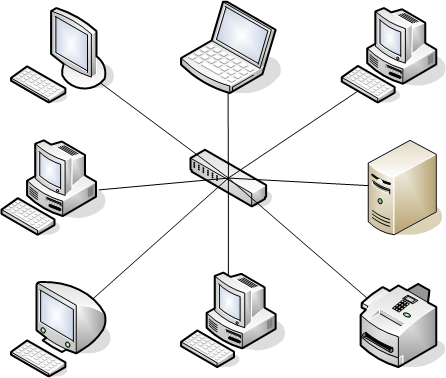
\includegraphics[width=0.4\linewidth]{img/Star_Topology.png}
    \caption{Mô hình dạng sao}
\end{figure}
Mạng dạng hình sao bao gồm một trung tâm và các nút thông tin. Các nút thông tin là các trạm đầu cuối, các máy tính và các thiết bị mạng khác. Trung tâm của mạng điều phối mọi hoạt động trong mạng với các chức năng cơ bản là:

\begin{itemize}[left=2cm]
    \item  Xác định cặp địa chỉ gửi và nhận được phép chiếm tuyến thông tin và liên lạc với nhau.
    \item Cho phép theo dõi và xử lý sai trong quá trình trao đổi thông tin.
\end{itemize}

\textbf{\textit{Mô hình dạng vòng (Ring Topology)}}

\begin{figure}[htbp]
    \centering
    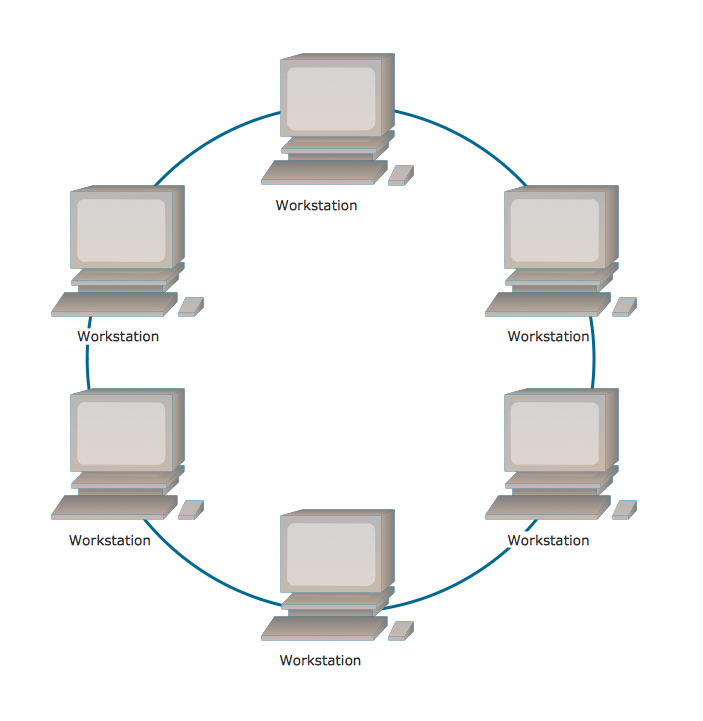
\includegraphics[width=0.4\linewidth]{img/Ring-Topology.png}
    \caption{Mô hình dạng vòng}
\end{figure}

Mạng dạng vòng được bố trí theo xoay vòng, đường dây cáp được thiết kế làm thành một vòng khép kín, tín hiệu chạy quanh theo một chiều nào đó. Các nút truyền cho nhau mỗi thời điểm chỉ được một nút. Dữ liệu truyền đi phải có kèm theo địa chỉ cụ thể của mỗi trạm tiếp nhận.
\newpage
\textbf{\textit{Mô hình dạng tuyến (Bus Topology)}}

\begin{figure}[htbp]
    \centering
    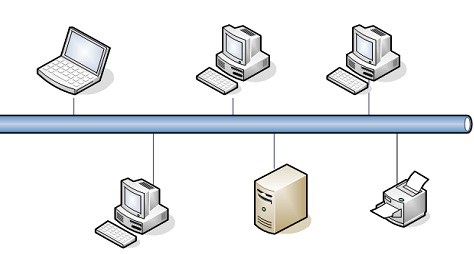
\includegraphics[width=0.5\linewidth]{img/bus-topology.jpeg}
    \caption{Mô hình dạng tuyến}
\end{figure}

Theo cách bố trí hành lang các đường như hình vẽ thì máy chủ (host) cũng như tất cả các máy tính khác (workstation) đều được nối về với nhau trên một trục đường dây cáp chính để chuyển tín hiệu. Tất cả các nút đều sử dụng chung đường dây cáp chính này. Phía hai đầu dây cáp được bịt bởi một thiết bị gọi là terminator. Các tín hiệu và gói dữ liệu khi di chuyển lên hoặc xuống trong dây cáp đều mang theo điạ chỉ của nơi đến.
\subsection*{1.2.3 Mô hình VXLAN}
\addcontentsline{toc}{subsection}{1.2.3 Mô hình VXLAN}

VXLAN (Virtual Extensible LAN) là một công nghệ mạng được thiết kế để giải quyết các vấn đề về mở rộng và linh hoạt trong mạng LAN truyền thống. VXLAN cho phép mở rộng một mạng LAN ở tầng 2 bằng cách sử dụng cơ sở hạ tầng mạng ở tầng 3. 

VXLAN được định nghĩa bởi IETF trong RFC 7348 và sử dụng kỹ thuật đóng gói để tạo ra các mạng ảo trên cùng một mạng vật lý. VXLAN mang lại nhiều lợi ích khi quyết định chọn triển khai:

\begin{itemize}[left=2cm]
    \item Mở rộng mạng ảo: Hỗ trợ lên đến 16 triệu mạng ảo, vượt xa giới hạn 4,096 VLAN.
    \item Hoạt động trên Layer 3: Kết nối mạng Layer 2 qua mạng IP, không phụ thuộc khoảng cách vật lý.
    \item Giảm vấn đề STP: Không cần Spanning Tree Protocol, tối ưu hóa sử dụng băng thông.
    \item Hỗ trợ đa thuê bao: Cô lập lưu lượng, tăng bảo mật và phù hợp cho môi trường đám mây.
    \item Tối ưu hiệu suất: Tận dụng ECMP, tăng băng thông và cân bằng tải.
    \item Tích hợp SDN: Quản lý linh hoạt và tự động hóa mạng dễ dàng.
\end{itemize}

Đây là một giải pháp lý tưởng cho các trung tâm dữ liệu quy mô lớn, môi trường đám mây, và các tổ chức cần mạng ảo hóa an toàn, mạnh mẽ, và có khả năng mở rộng vượt trội để đáp ứng nhu cầu ngày càng cao trong kỷ nguyên công nghệ số.

\subsection*{1.2.4 Các giao thức}
\addcontentsline{toc}{subsection}{1.2.4 Các giao thức}

\textbf{\textit{HSRP (Hot Standby Router Protocol)}}

HSRP là một giao thức dự phòng của Cisco, được sử dụng để cung cấp tính khả dụng cao cho các gateway mặc định trong mạng. Giao thức có một số đặc điểm chính:

\begin{itemize}[left=2cm]
    \item Đảm bảo rằng nếu một router hoặc gateway gặp sự cố, một router khác sẽ tự động thay thế mà không làm gián đoạn lưu lượng.
    \item Cung cấp một địa chỉ IP hoặc MAC ảo mà các thiết bị trong mạng sử dụng làm gateway mặc định.
    \item Khi xử lý 1 lưu lượng mạng, một router sẽ chờ trong trạng thái dự phòng và sẽ hoạt động nếu router chính thất bại.
\end{itemize}

\textbf{\textit{OSPF (Open Shortest Path First)}}

OSPF là một giao thức định tuyến động link-state được sử dụng trong các mạng IP để tìm đường tốt nhất dựa trên thuật toán Dijkstra. Có các đặc điểm như sau:

\begin{itemize}[left=2cm]
    \item Cung cấp khả năng định tuyến động và tự động thích nghi khi xảy ra thay đổi trong mạng.
    \item Là giao thức mở, không thuộc độc quyền của bất kỳ hãng nào (RFC 2328).
    \item Tìm đường đi tối ưu trong mạng IP và tự động cập nhật khi mạng thay đổi.
    \item Phù hợp cho mạng lớn, phân vùng theo Area.
\end{itemize}

\textbf{\textit{STP (Spanning Tree Protocol)}}

STP là một giao thức được sử dụng để ngăn chặn các vòng lặp trong mạng Ethernet và đảm bảo một đường dẫn duy nhất giữa các switch. Đặc điểm chính:

\begin{itemize}[left=2cm]
    \item Giao thức ngăn vòng lặp trong mạng Ethernet (Layer 2).
    \item Đảm bảo có một đường dẫn duy nhất trong mạng switch.
    \item Tất cả các switch trong mạng bầu chọn một switch làm Root Bridge dựa trên Bridge ID (ưu tiên thấp nhất sẽ thắng).
    \item STP gửi các gói BPDU để trao đổi thông tin và duy trì cấu trúc cây.
\end{itemize}
\subsection*{1.2.5 Mạng ảo VPN}
\addcontentsline{toc}{subsection}{1.2.5 Mạng ảo VPN}

VPN là sự mở rộng của một mạng riêng thông qua các mạng công cộng. Về cơ bản, mỗi VPN là một mạng riêng rẽ sử dụng một mạng chung (thường là Internet) để kết nối cùng với các site hay nhiều người sử dụng từ xa. Thay cho việc sử dụng kết nối thực, mỗi VPN sử dụng các kết nối ảo được dẫn qua đường Internet từ mạng riêng của các công ty tới các site, nhân viên từ xa. Công nghệ VPN có thể được phân thành 2 loại cơ bản: 
\begin{itemize}[left=2cm]
    \item \textbf{Site-to-Site VPN:} là mô hình dùng để kết nối các hệ thống mạng ở các nơi khác nhau tạo thành một hệ thống mạng thống nhất.
    \item \textbf{Remote Access VPN:} loại này thường áp dụng cho nhân viên làm việc lưu động hay làm việc ở nhà muốn kết nối vào mạng công ty một cách an toàn. Cũng có thể áp dụng cho văn phòng nhỏ ở xa kết nối vào Văn phòng trung tâm của công ty.
\end{itemize}

Mô hình VPN có nhiều lợi ích như sau:

\begin{itemize}[left=2cm]
    \item Chi phí thấp: chi phí thiết lập mạng VPN thấp hơn so với các mạng WAN truyền thống như Frame Relay, ATM, Leased Line.
    \item Tăng cường tính bảo mật: sử dụng các giao thức đóng gói, các thuật toán mã hóa và các phương pháp chứng thực để bảo mật dữ liệu trong quá trình truyền.
    \item Tính mở rộng và linh động: VPN đã xóa bỏ rào cản về mặt địa lý cho hệ thống mạng, sẵn sàng kết nối các mạng riêng lại với nhau một cách dễ dàng thông qua môi trường Internet.
\end{itemize}
